
\section{Controller Analysis}\label{ssec:ControllerVerification}
A further analysis can be done to the controller, both continuous and discrete, and also to the real response of the system once it is implemented.
A first approach is to simulate the continuous controller and see how the system behaves with it.

With a constant reference of 0 rad and a disturbance in the form of an small initial angle (\si{0,001 rad}) the response is the one shown in figref{} and figref{}.

\fxnote{Include response of the continuous controller, both torque and position}

It is also necessary to verify that the discretized controller matches the original continuous one, and is also able to maintain the Cubli in the upright position. This is done firstly, by simulating the feedback system and comparing the newly made discrete controller with the continuous simulation from figref{fig:continuousControllerSimulation}, see \figref{fig:discreteVsContinuousSimulation}.
%

  \begin{minipage}{0.45\linewidth}
    \begin{figure}[H]
      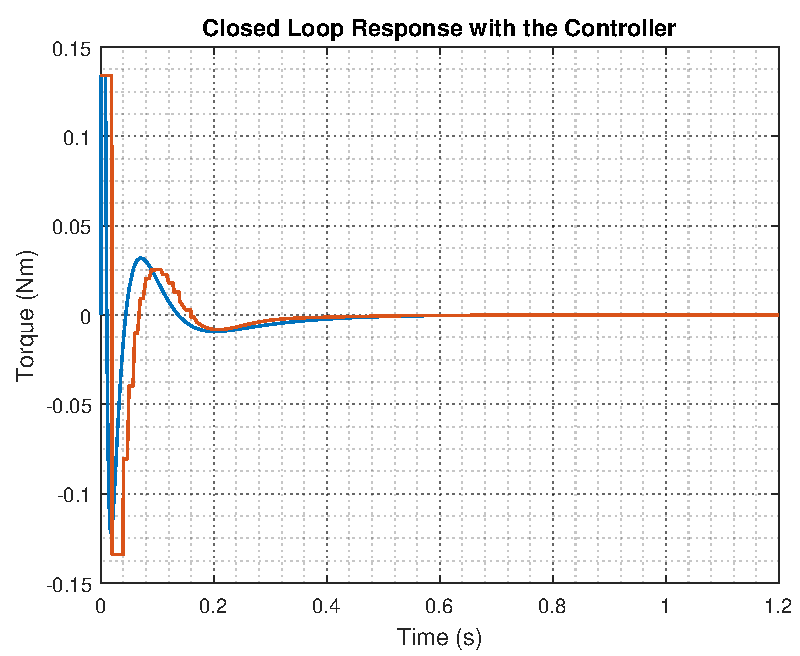
\includegraphics[scale=.53]{figures/torqueComp.pdf}
      \captionsetup{justification=centering}
      \captionof{figure}{Controller's output (torque) response in the control loop with the continuous (blue) and discrete (red) controllers}
      \label{fig:discreteVsContinuousOutputController}
    \end{figure}\vspace{-5mm}
  \end{minipage}
  \hspace{0.03\linewidth}
  \begin{minipage}{0.45\linewidth}
    \begin{figure}[H]\vspace{-9mm}
      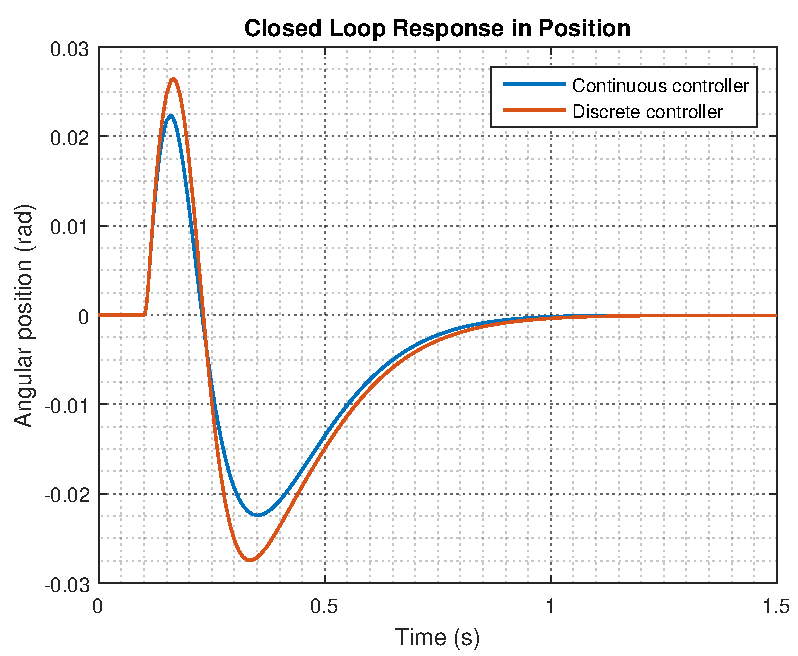
\includegraphics[scale=.53]{figures/positionComp.pdf}
      \captionsetup{justification=centering}
      \captionof{figure}{Closed loop response of the continuous (blue) and discrete (red) controllers}
      \label{fig:discreteVsContinuousSimulation}
    \end{figure}\vspace{-5mm}
  \end{minipage}


In \figref{discreteVsContinuousSimulation}, the system is given an initial condition of. The discretized controller seems to fulfill the basic requirement of putting back the Cubli in the upright (\si{0^{\circ}}) position. However, ...